\documentclass[a4paper, 11pt]{article}
 
\usepackage{VB}

%\doublespacing

\begin{document}

%\lhead{\textsc{Virtual paper - Public economics and development - Vincent Bagilet}}

\selectlanguage{english}
	
	\title{Unconfounded but inflated causal estimates}
	\subtitle{Mathematical description}

	\author{Vincent Bagilet, Léo Zabrocki}
	
	%\institution{Columbia University}

	\date{\today}
	
	\maketitle
	
	\section{Setting}
	
		\subsection{Objectives}\label{maths_objectives}
	
		This document aims to provide a mathematical derivation to illustrate the trade-off underlined in this paper. Such a derivation may provide some intuition regarding the various mechanisms at play. It does not aim in any way to provide a general proof but merely a specific one, tied to the setting considered. While we keep this setting as general as possible, as in most cases, we have to make certain assumptions, in particular regarding the data generating process considered. 
		
		The objective here is to compare the exaggeration ratio for a naive regression with omitted variable bias (OVB) to that of an Instrumental Variable (IV) model in which we instrument the variable affected by the omitted variable. We expect the naive regression to be biased but more precise than the IV and therefore less subject to exaggeration problems. Roughly, we aim to derive the conditions under which the exaggeration due to the loss in precision is greater than the OVB. %The following simulation illustrates this in the case of the 
		Thus, the objective is to compare the following quantities:
			\begin{gather*}
				\mathbb{E}\left[ \hat{\beta}_{\textsc{ovb}} | \beta_{1}, b_{\textsc{ovb}}, \sigma_{\textsc{ovb}}, \hat{\beta}_{\textsc{ovb}} > z_{\alpha} \sigma_{\textsc{ovb}} \right] \\
				%\mathbb{E}\left[ \hat{\beta}_{\textsc{r}} | \beta_{0}, \sigma_{\textsc{r}}, \hat{\beta}_{\textsc{r}} > z_{\alpha} \sigma_{\textsc{r}} \right]\\
				\mathbb{E}\left[ \hat{\beta}_{\textsc{iv}} | \beta_{1}, \sigma_{\textsc{iv}}, \hat{\beta}_{\textsc{iv}} > z_{\alpha} \sigma_{\textsc{iv}} \right]
			\end{gather*} 
			
			where \textsc{ovb} and \textsc{iv} denote the naive regression and the IV respectively. $\beta_{1}$ represents the true effect of interest, $\hat{\beta_{..}}$ its estimate, $\sigma_{..}$ the standard error of the estimate and $z_{\alpha}$ the threshold value of a two-sided test of size $\alpha$.% and $b_{\textsc{..}}$ the bias in the naive regression. Note that due to the exogeneity assumption $b_{\textsc{iv}} = 0$. 
			
			To compute these values, we need to know the distribution of the estimates. After describing the data generating process, we thus derive the asymptotic distribution of these estimates. We then compute and compare these quantities as a function of the parameters of interests. The main parameter of interest is linked the proportion of the variance in the explanatory variable of interest retained for identification. 
				
		\subsection{Data generating process}\label{maths_dgp}
			%I build this using the notation used by Dong Woo in his lecture notes
		
			Consider the usual linear regression model to which we add omitted variables. We limit the number of covariates considered to a constant, an observed variable and an omitted variable. For all individual $i \in {1, ..., n}$, we make the following assumptions: 
			
				\begin{equation}\label{maths_true_dgp}
					y_i = \text{x}_i' \bm{\beta} + \delta w_{i} + u_i
				\end{equation}
				
				where $\text{x}_i \in \mathbb{R}^2$ is a vector including a constant and the observed explanatory variable such that $\text{x}_i = (1, x_i)'$, $y_i \in \mathbb{R}$ the observed outcome of interest, $w_i \in \mathbb{R}$ an unobserved omitted variable, $u_i \in \mathbb{R}$ an unobserved error term. $\bm{\beta} \in \mathbb{R}^{2}$ and $\delta \in \mathbb{R}$ are unknown parameters. $\bm{\beta} = (\beta_0, \beta_1)'$ and $\beta_1$ is the parameter of interest. For readability, we introduce the usual vector notation such that for instance $y = (y_1, ..., y_n)'$. 
			
			We further assume that the usual OLS assumptions hold: ($y_i, \text{x}_i, w_{i}, u_{i}$) are iid, finite second moments, \textit{ie} $\mathbb{E}[y_{i}^{2}] < \infty$, $\mathbb{E}[w_{i}^{2}] < \infty$, $\mathbb{E}[x_{i}^{2}] < \infty$, positive-definiteness of $\mathbb{E}[\text{x}_i \text{x}_i']$, $u_{i}$ is conditional mean-zero, \textit{ie} $\mathbb{E}[u_{i} | x_{i}, w_{i}] = 0$, and is uncorrelated with $x_i$ and $w_i$, \textit{ie} $\mathbb{E}[x_{i}u_{i}] = 0$ and $\mathbb{E}[w_{i}u_{i}] = 0$. Note that conditional mean-zero implies that $\mathbb{E}[u_{i} | x_{i}] = 0$ (since $\mathbb{E}[u_{i} | x_{i}] = \mathbb{E}[\mathbb{E}[u_{i} | x_{i}, w_{i}| x_{i}]]  = \mathbb{E}[0 | x_{i}] = 0$). We further assume homoskedasticity such that $\mathbb{E}[u_i^{2} | x_{i}, w_{i}] = \sigma_{u}^{2}$ is constant. It implies that  $\mathbb{E}[u_i^{2} | x_{i}] = \sigma_{u}^{2}$ (since $\mathbb{E}[u_i^{2} | x_{i}] =  \mathbb{E}[\mathbb{E}[u_i^{2} | x_{i}, w_{i}]|x_{i}] = \mathbb{E}[\sigma_{u}^{2} | x_{i}] = \sigma_{u}^{2})$.
			
			We however assume that $w_{i}$ is unobserved, correlated with $x_{i}$ and that $\delta \neq 0$. To simplify the derivations, we further assume that the unobserved variable is centred, \textit{ie} $\mathbb{E}[w_i] = 0$. We also assume that the variance of the component of $w_{i}$ that is orthogonal to $x_{i}$ (denoted $w_{i}^{\perp}$) does not vary with $x_{i}$. Thus, $\text{Var}(w_{i}^{\perp}|x_{i}) = \text{Var}(w_{i}^{\perp})$.
			
			We further assume that there exists a valid instrumental variable $z_i$ for $x_i$. Let $\text{z} = (1, z_i)' \in \mathbb{R}^{2}$. Note that the model is just-identified. Since the instrument is valid, it satisfies exogeneity, \textit{ie} $\mathbb{E}[\text{z}_{i}u_{i}] = 0$ and  $\mathbb{E}[z_{i}w_{i}] = 0$, relevance, \textit{ie} $\text{rank}(\mathbb{E}[\text{z}_{i}\text{x}_i']) = 2$,  and positive-definiteness of $\mathbb{E}[\text{z}_i \text{z}_i']$. To simplify interpretation, we further assume a data generating process for $x_i$:			
				~
				\begin{equation}\label{maths_dgp_x}
					x_i = \eta_0 + \eta_1 z_i + \gamma w_{i} + \epsilon_i
				\end{equation}
				
				where $(\eta_0, \eta_1, \gamma) \in \mathbb{R}^{3}$ are unknown parameters. We assume that $\epsilon_i$ is uncorrelated with $z_i$ and $w_{i}$, \textit{ie} $\mathbb{E}[z_i\epsilon_i] = 0$ and $\mathbb{E}[w_i\epsilon_i] = 0$. Note that, since $x_i$ and $w_i$ are correlated, $\gamma \neq 0$.\\
				
				%We assumed that the coefficient for $d$ in equation \ref{maths_dgp_x} is unitary to be able to compare $\beta_{\textsc{R}}$, the coefficient for $d$ in the reduced form regression (regressing $y$ on $d$), to $\beta_{\textsc{ovb}}$, the coefficient for $x$ in the naive regression (regressing $y$ on $x$).  Roughly, $\beta_{\textsc{ovb}}$ can be interpreted as the variation in $y$ associated with a variation of $x$ by one. Similarly, $\beta_{\textsc{R}}$ can be interpreted as the variation in $y$ associated with a variation of $d$ by one. A variation in $d$ by one causes a variation of $x$ by one. Thus, both $\beta_{\textsc{ovb}}$ and $\beta_{\textsc{R}}$ can be interpreted as the variation in $y$ associated with a variation of $x$ by one. They are however different since this variation is orthogonal to the unobserved variable in the case of the reduced form but not in the case of the naive regression.\\
				
				The following Directed Acyclic Graph (DAG) sums up the relationships between the variables. It also helps underline the independence, or not, of some variables. 
				
				\begin{figure}[!h] 
            					\begin{center}
            						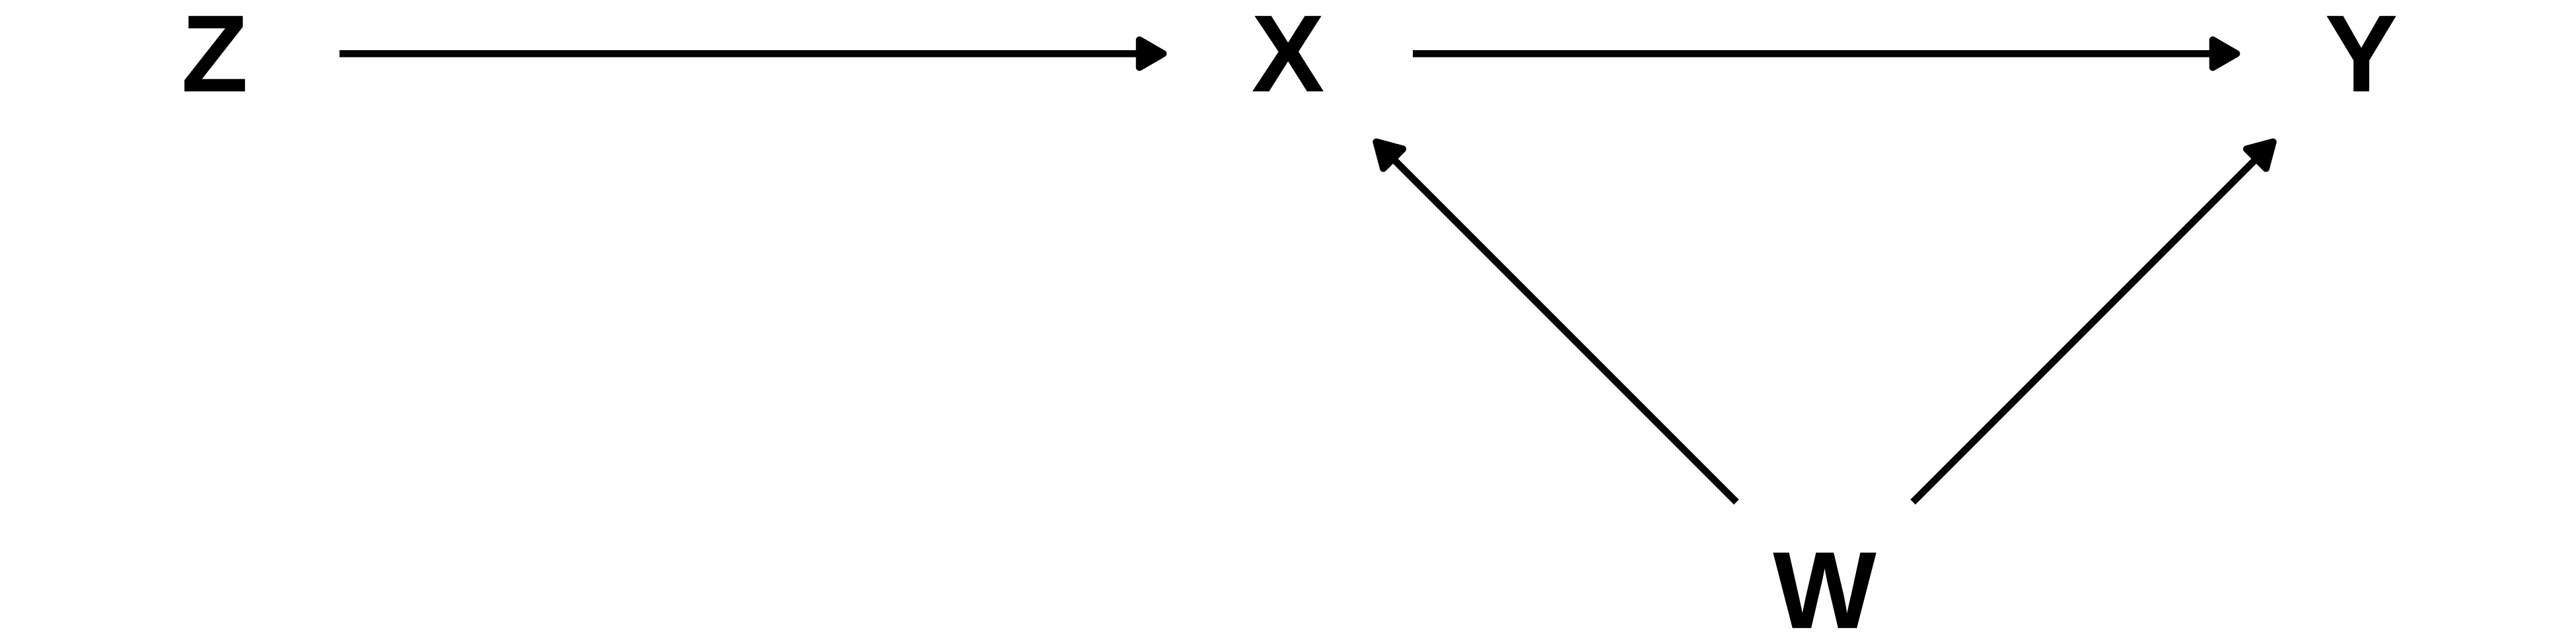
\includegraphics[width=8cm]{../images/DAG_maths-1.png}
            						\caption{DAG of the data generating process}
            						\label{maths_dag_dgp}
            					\end{center}
            				\end{figure} 
				\vspace{-0.8cm}
	
			
				
						
		\subsection{Summary of the key assumptions}
		
			To ease the use of assumptions in the following sections, we summarize some that we will explicitly mobilize:
		 
			\begin{itemize}
				\item $y_i = \text{x}_i' \bm{\beta} + \delta w_{i} + u_i$
				\item $x_i = \eta_0 + \eta_1 z_i + \gamma w_{i} + \epsilon_i$
				\item $\mathbb{E}[u_{i} | x_{i}, w_{i}] = 0$ and $\mathbb{E}[u_{i} | x_{i}] = 0$
				\item $\mathbb{E}[u_i^{2} | x_{i}, w_{i}] = \sigma_{u}^{2}$ and $\mathbb{E}[u_i^{2} | x_{i}] = \sigma_{u}^{2}$
				\item $\mathbb{E}[w_i] = 0$
				\item $\mathbb{E}[z_{i}u_{i}] = 0$ and $\mathbb{E}[z_{i}w_{i}] = 0$
				\item $\mathbb{E}[z_i\epsilon_i] = 0$ and $\mathbb{E}[w_i\epsilon_i] = 0$
				\item $\text{Var}(w_{i}^{\perp}|x_{i}) = \text{Var}(w_{i}^{\perp})$
			\end{itemize}

%%%%%%%%%%%%%%%%%%%%%%%%%%%%%%%%%%%%%%%%%%%

	\section{Asymptotic distribution of the estimates}
	
		As discussed above, the goal is to compare the exaggeration ration in the case of the naive regression to that of the corresponding reduced form and IV. In this section, we \textbf{derive the asymptotic distributions of these estimates}.

%%%%%%%%%%%%%%%%%%%%%%%%%%%%%%%%%%%%%%%%%%%	
		
		\subsection{Naive regression (OVB)}
			
			The true DGP is given by equation \ref{maths_true_dgp}. Since, we do not observe $W$, we consider the projection of $y$ on $X$ only:
				
				\begin{equation}\label{maths_eq_ovb}
					y = X\bm{\beta}_{\textsc{ovb}} + v
				\end{equation}
				
				where $v = (v_{1}, ... , v_{n})' \in \mathbb{R}^{n}$ and by definition of the projection, $\mathbb{E}[X'v] = 0$.
				
			\subsubsection{Bias of the estimator}
				
				From equation  \ref{maths_eq_ovb} we get: 
				~
				\begin{align*}
					& X'y = X'X\bm{\beta}_{\textsc{ovb}} + X'v\\
					\Rightarrow \quad & \mathbb{E}[X'y] = \underbrace{\mathbb{E}[X'X]}_{\text{pos. def.}}\bm{\beta}_{\textsc{ovb}} + \underbrace{\mathbb{E}[X'v]}_{0} \\
					\Leftrightarrow \quad & \bm{\beta}_{\textsc{ovb}} = \mathbb{E}[X'X]^{-1} \mathbb{E}[X'y]\\
					\Leftrightarrow \quad & \bm{\beta}_{\textsc{ovb}} = \mathbb{E}[X'X]^{-1} \mathbb{E}[X'(X\bm{\beta} + \delta w + u)] & \text{cf eq. \ref{maths_true_dgp}}\\
					\Leftrightarrow \quad & \bm{\beta}_{\textsc{ovb}} = \bm{\beta} + \mathbb{E}[X'X]^{-1} \mathbb{E}[X'w] \delta + \underbrace{\mathbb{E}[X'u]}_{0}\\
					\Leftrightarrow \quad & \bm{\beta}_{\textsc{ovb}} = \bm{\beta} + \mathbb{E}[X'X]^{-1} \mathbb{E}[X'w] \delta
				\end{align*}		
				
				Since $X$ and $w$ are correlated and $\delta \neq 0$, $\boxed{\bm{\beta}_{\textsc{ovb}} \neq \bm{\beta}}$. $ \mathbb{E}[X'X]^{-1} \mathbb{E}[X'w]$ is the coefficient matrix of the projection of $w$ on $X$. A similar derivation and discussion is carried out in \cite{hansen_econometrics_2022} for instance.\\ %p 43
				
				Let $\hat{\bm{\beta}}_{\textsc{ovb}}$ denote the least square estimator of $\bm{\beta}_{\textsc{ovb}}$. We thus have:
				~
				\begin{equation}
					\hat{\bm{\beta}}_{\textsc{ovb}} = (X'X)^{-1}X'y
				\end{equation}
				\begin{align*}
					\Rightarrow \quad  & \hat{\bm{\beta}}_{\textsc{ovb}} = (X'X)^{-1}X'(X\bm{\beta}_{\textsc{ovb}} + v) & \text{cf eq. \ref{maths_eq_ovb}}\\
					\Rightarrow \quad  & \mathbb{E}[\hat{\bm{\beta}}_{\textsc{ovb}} | X] = \bm{\beta}_{\textsc{ovb}} + (X'X)^{-1}\underbrace{\mathbb{E}[X'v]}_{0} \\
					\Rightarrow \quad  & \mathbb{E}[\hat{\bm{\beta}}_{\textsc{ovb}}] = \mathbb{E}[\mathbb{E}[\hat{\bm{\beta}}_{\textsc{ovb}} | X]] = \bm{\bm{\beta}}_{\textsc{ovb}}& \text{by the Law of Iterated Expect. (LIE)} 
				\end{align*}
				
				Thus, \underline{$\hat{\bm{\beta}}_{\textsc{ovb}}$ is an unbiased estimator of $\bm{\beta}_{\textsc{ovb}}$ but a biased estimator of $\bm{\beta}$}. We then compute its asymptotic distribution. 
				
			\subsubsection{Asymptotic distribution}	
				
				We can write: 
				~
				\begin{align*}
					\sqrt{n}(\hat{\bm{\beta}}_{\textsc{ovb}} - \bm{\beta}_{\textsc{ovb}}) &  = \left(\dfrac{1}{n} \sum_{i = 1}^{n} \text{x}_{i} \text{x}_{i}' \right)^{-1} \sqrt{n} \left(\dfrac{1}{n} \sum_{i = 1}^{n} \text{x}_{i} v_{i} \right)
				\end{align*}	
				
				By the Weak Law of Large Numbers (WLLN), $\dfrac{1}{n} \sum_{i = 1}^{n} \text{x}_{i} \text{x}_{i}'  \overset{p}{\to}  \mathbb{E}[\text{x}_{i}\text{x}_{i}']$. 
				
				Since $\mathbb{E}[\text{x}_{i}v_{i}] = 0$, by the Central Limit Theorem (CLT), $\sqrt{n} \left(\dfrac{1}{n} \sum_{i = 1}^{n} \text{x}_{i} v_{i} \right) \overset{d}{\to} \mathcal{N}(0, \mathbb{E}[\text{x}_{i}\text{x}_{i}'v_{i}^{2}])$. 
				
				Applying Slutsky's theorem then yields:
				
				\[ \sqrt{n}(\hat{\bm{\beta}}_{\textsc{ovb}} - \bm{\beta}_{\textsc{ovb}}) \overset{d}{\to} \mathcal{N}\left(0,  \mathbb{E}[\text{x}_{i}\text{x}_{i}']^{-1} \mathbb{E}[\text{x}_{i}\text{x}_{i}'v_{i}^{2}] \mathbb{E}[\text{x}_{i}\text{x}_{i}']^{-1}\right) \]
				
				And thus,
				~
				\begin{equation}\label{asympt_ovb}
					\boxed{
						\hat{\bm{\beta}}_{\textsc{ovb}} \overset{d}{\to} \mathcal{N}\left( \bm{\beta} + \mathbb{E}[\text{x}_{i}\text{x}_{i}']^{-1} \mathbb{E}[\text{x}_{i} w_{i}] \delta ,  \mathbb{E}[\text{x}_{i}\text{x}_{i}']^{-1} \mathbb{E}[\text{x}_{i}\text{x}_{i}'v_{i}^{2}] \mathbb{E}[\text{x}_{i}\text{x}_{i}']^{-1} / n \right) 
					}
				\end{equation}
				
				We are interested in the second component of $\hat{\bm{\beta}}_{\textsc{ovb}}$. To retrieve it we need to compute $\mathbb{E}[\text{x}_{i}\text{x}_{i}']^{-1}$, $ \mathbb{E}[\text{x}_{i} w_{i}] $ and $\mathbb{E}[\text{x}_{i}\text{x}_{i}'v_{i}^{2}]$.  
				
				\[ 
				\mathbb{E}[\text{x}_{i}\text{x}_i'] 
				= \mathbb{E} \begin{bmatrix}
					1 & x\\ 
					x & x^{2}
				\end{bmatrix} 
				=
				\begin{bmatrix}
					1 & \mu_{x}\\ 
					\mu_{x} & \sigma_{x}^{2} + \mu_{x}^2
				\end{bmatrix} 
				\quad \Rightarrow \quad
				     \mathbb{E}[\text{x}_{i}\text{x}_i']^{-1} = \dfrac{1}{\sigma_{x}^{2}} 
				     									\begin{bmatrix}
														 \sigma_{x}^{2} + \mu_{x}^2 & -\mu_{x}\\ 
														-\mu_{x} & 1
													\end{bmatrix} 
				\]
				
				\begin{equation*} 
            				\mathbb{E}[\text{x}_{i}w_i] = 
            				\mathbb{E}
            					\begin{bmatrix}
            						w_i\\ 
            						x_iw_i
            					\end{bmatrix} 
            				=
            				\begin{bmatrix}
            				    	0\\ 
            					\mathbb{E}[x_{i}]\underbrace{\mathbb{E}[w_{i}]}_{0} + \text{cov}(x_{i}, w_{i}) 
            				\end{bmatrix} 
            				= 
            				\begin{bmatrix}
            				    	0\\ 
            					\eta_1 \underbrace{\text{cov}(z_{i}, w_{i})}_{0} + \gamma  \underbrace{\text{var}(w_{i})}_{\sigma_{w}^{2}} + \underbrace{\text{cov}(\epsilon_{i}, w_{i})}_{0} 
            				\end{bmatrix} 
            				=
            				\begin{bmatrix}
            				    	0\\ 
            					\gamma \sigma_{w}^{2}
            				\end{bmatrix} 
				\end{equation*}
				
				\begin{equation}\label{bias_ovb}
					\Rightarrow \quad
					\mathbb{E}[\text{x}_{i}\text{x}_i']^{-1}\mathbb{E}[\text{x}_{i}w_i] 
					=
					\dfrac{\gamma\sigma_{w}^{2}}{\sigma_{x}^{2}}
					\begin{bmatrix}
				    		- \mu_{x} \\
						1
					\end{bmatrix} 
				\end{equation}
				
				Note that $\mathbb{E}[\text{x}_{i}\text{x}_{i}'v_{i}^{2}] \overset{\textsc{lie}}{=} \mathbb{E}[\text{x}_{i}\text{x}_{i}'\mathbb{E}[v_{i}^{2} | \text{x}_{i}]]$. We thus first compute $\mathbb{E}[v_{i}^{2} | \text{x}_{i}]$, noting that:
				~
				\begin{align*}
            				v_i & =  y_i - \text{x}_i'\bm{\beta}_{\textsc{ovb}} \\
            					& = \delta w_{i} + u_i + \text{x}_i' (\bm{\beta} - \bm{\beta}_{\textsc{ovb}})\\
            					& = \delta w_{i} + u_i - \underbrace{\text{x}_{i}' \mathbb{E}[\text{x}_{i}\text{x}_{i}']^{-1} \mathbb{E}[\text{x}_{i}w_{i}]}_{\text{projection of $w_i$ on $x_i$}} \delta\\
            					& =  u_i + \delta \underbrace{\left(w_{i} - \dfrac{\gamma\sigma_{w}^{2}}{\sigma_{x}^{2}} (x_{i} - \mu_{x})\right)}_{\text{part of $w_i$ orthogonal to $x_i$}}\\
						& = u_i + \delta w_{i}^{\perp} & \text{where } w_{i}^{\perp} = w_{i} - \dfrac{\gamma\sigma_{w}^{2}}{\sigma_{x}^{2}} (x_{i} - \mu_{x})
				\end{align*}
				
				And thus,
				\begin{align*}
            				\mathbb{E}[v_{i}^{2} | \text{x}_{i}] & = \mathbb{E}[(u_i + \delta w_{i}^{\perp})^{2}| x_{i}]\\
					& = \mathbb{E}[u_{i}^{2} | x_{i}] + 2\delta \mathbb{E}[u_{i}w_{i}^{\perp} | x_{i}] + \delta^{2}\mathbb{E}[(w_{i}^{\perp})^{2} | x_{i}]\\
					& = \sigma_{u}^{2} + 2\delta \left( \mathbb{E}[u_{i}w_{i} | x_{i}] -  \dfrac{\gamma\sigma_{w}^{2}}{\sigma_{x}^{2}} (x_{i} - \mu_{x})\underbrace{\mathbb{E}[u_{i}|x_{i}]}_{0} \right) + \delta^{2}\mathbb{E}[(w_{i}^{\perp})^{2} | x_{i}]\\
					& \overset{\textsc{lie}}{=} \sigma_{u}^{2} + 2\delta \mathbb{E}[w_{i} \underbrace{\mathbb{E}[u_{i} | x_{i}, w_{i}]}_{0} | x_{i}] + \delta^{2}\mathbb{E}[(w_{i}^{\perp})^{2} | x_{i}]\\
					& = \sigma_{u}^{2} +  \delta^{2}\mathbb{E}[(w_{i}^{\perp})^{2} | x_{i}]
				\end{align*}
				
				Notice that, by the law of total variance, $\mathbb{E}[(w_{i}^{\perp})^{2} | x_{i}] = \text{Var}(w_{i}^{\perp} | x_{i}) + \mathbb{E}[w_{i}^{\perp} | x_{i}]^{2}$. Now, since $w_{i}^{\perp}$ is the component of $w_{i}$ that is orthogonal to $x_{i}$ and by the projection interpretation of the conditional variance,  $\mathbb{E}[w_{i}^{\perp} | x_{i}] = 0$. And thus, since by assumption $\text{Var}(w_{i}^{\perp} | x_{i}) = \text{Var}(w_{i}^{\perp})$, 
				~
				\begin{align*}
					\mathbb{E}[(w_{i}^{\perp})^{2} | x_{i}] & = \text{Var}(w_{i}^{\perp} | x_{i})\\
					& = \text{Var}(w_{i}^{\perp}) \\
					& = \mathbb{E}[(w_{i}^{\perp})^{2}] - \mathbb{E}[w_{i}^{\perp}]^{2}\\
					& = \mathbb{E}\left[ \left(w_{i} - \dfrac{\gamma\sigma_{w}^{2}}{\sigma_{x}^{2}} (x_{i} - \mu_{x})\right)^{2} \right] - \left(\underbrace{\mathbb{E}[w_{i}]}_{0} + \dfrac{\gamma\sigma_{w}^{2}}{\sigma_{x}^{2}} \underbrace{\mathbb{E}[x_{i} - \mu_{x}]}_{0} \right)^{2}\\
					& = \underbrace{\mathbb{E}[w_{i}^{2}]}_{\sigma_{w}^{2}} - 2 \dfrac{\gamma\sigma_{w}^{2}}{\sigma_{x}^{2}} \left( \underbrace{\mathbb{E}[x_{i}w_{i}]}_{\gamma \sigma_{w}^{2}} - \mu_{x}\underbrace{\mathbb{E}[w_{i}]}_{0} \right) + \dfrac{\gamma^{2}\sigma_{w}^{4}}{\sigma_{x}^{4}} \underbrace{\mathbb{E}[(x_{i} - \mu_{x})^{2}]}_{\sigma_{x}^{2}}\\
					& = \sigma_{w}^{2} - 2 \dfrac{\gamma^{2}\sigma_{w}^{4}}{\sigma_{x}^{2}} + \dfrac{\gamma^{2}\sigma_{w}^{4}}{\sigma_{x}^{2}}\\
					& = \sigma_{w}^{2} - \dfrac{\gamma^{2}\sigma_{w}^{4}}{\sigma_{x}^{2}} \\
					& = \sigma_{w}^{2} \left(1 - \dfrac{\gamma^{2}\sigma_{w}^{2}}{\sigma_{x}^{2}} \right)
				\end{align*}
				
				And therefore, 
				~
				\begin{equation}
					\mathbb{E}[v_{i}^{2} | \text{x}_{i}] =  \sigma_{u}^{2} +  \delta^{2} \sigma_{w}^{2} \left(1 - \dfrac{\gamma^{2}\sigma_{w}^{2}}{\sigma_{x}^{2}} \right)
				\end{equation}
				
				Thus, under our set of assumptions, $\mathbb{E}[v_{i}^{2} | \text{x}_{i}]$ does not depend on $x_{i}$ and $\mathbb{E}[v_{i}^{2} | \text{x}_{i}] =  \mathbb{E}[v_{i}^{2}]$. We denote this quantity $\sigma_{v}^{2}$. \\
				
				We can now compute the variance of the estimator $\hat{\bm{\beta}}_{\textsc{ovb}}$, noting that $\mathbb{E}[\text{x}_{i}\text{x}_{i}'v_{i}^{2}] = \mathbb{E}[\text{x}_{i}\text{x}_{i}'\mathbb{E}[v_{i}^{2} | \text{x}_{i}]] =  \mathbb{E}[\text{x}_{i}\text{x}_{i}' \sigma_{v}^{2}] = \sigma_{v}^{2} \mathbb{E}[\text{x}_{i}\text{x}_{i}']$. 
				
				Thus, plugin this and equation \ref{bias_ovb} into equation \ref{asympt_ovb}, for $\hat{\beta}_{\textsc{ovb}}$, the second component of $\hat{\bm{\beta}}_{\textsc{ovb}}$, we have:
				\begin{equation}
						\hat{\beta}_{\textsc{ovb}} \overset{d}{\to} \mathcal{N}\left( \beta_1 + \dfrac{\delta \gamma \sigma_{w}^{2}}{\sigma_{x}^{2}}, \ \dfrac{\sigma_{v}^{2}}{n \ \sigma_{x}^{2}} \right) 
				\end{equation}
				
				And substituting for $\sigma_{v}^{2}$,
				\begin{equation}
					\boxed{
						\hat{\beta}_{\textsc{ovb}} \overset{d}{\to} \mathcal{N}\left( \beta_1 + \dfrac{\delta \gamma \sigma_{w}^{2}}{\sigma_{x}^{2}}, \ \dfrac{ \sigma_{u}^{2} +  \delta^{2} \sigma_{w}^{2} \left(1 - \frac{\gamma^{2}\sigma_{w}^{2}}{\sigma_{x}^{2}} \right)}{n \ \sigma_{x}^{2}} \right) 
					}
				\end{equation}
				
				Using the notations introduced in section \ref{maths_objectives}, we have:
				~
				\begin{align*}
					b_{\textsc{ovb}} & = \dfrac{\delta \gamma \sigma_{w}^{2}}{\sigma_{x}^{2}}\\
					\sigma_{\textsc{ovb}}^{2} & = \dfrac{ \sigma_{u}^{2} +  \delta^{2} \sigma_{w}^{2} \left(1 - \frac{\gamma^{2}\sigma_{w}^{2}}{\sigma_{x}^{2}} \right)}{n \ \sigma_{x}^{2}}
				\end{align*}				
				
				
				% LOOK AT DEMEANED VERSION IN HANSEN p 71!!!!!!
				
%%%%%%%%%%%%%%%%%%%%%%%%%%%%%%%%%%%%%%%%%%%	
		
		\subsection{Instrumental Variable}
			
			The true DGP for $y$ is given by equation \ref{maths_true_dgp}. Here, we instrument $x_{i}$ with $z_{i}$, or more precisely $\text{x}_{i} = (1, x_{i})'$ with $\text{z}_{i} = (1, z_{i})'$. We are therefore in a just-identified case and $\hat{\bm{\beta}}_{\textsc{2sls}} = \hat{\bm{\beta}}_{\textsc{iv}}$. And:
			~
			\begin{align*}
				 \hat{\bm{\beta}}_{\textsc{iv}} & =  (Z'X)^{-1}Z'y\\
				 	& = (Z'X)^{-1}Z'(X\bm{\beta} + \delta w + u)\\
				 	& = \bm{\beta} + (Z'X)^{-1}Z'w \delta + (Z'X)^{-1}Z'u
			\end{align*}
			
			Thus,
			~
			\begin{equation*}
				\mathbb{E}[ \hat{\bm{\beta}}_{\textsc{iv}} | X, Z]  =  \bm{\beta} + (Z'X)^{-1}\underbrace{\mathbb{E}[Z'w]}_{0} \delta + (Z'X)^{-1}\underbrace{\mathbb{E}[Z'u]}_{0} = \bm{\beta}
			\end{equation*}
			
			$\hat{\bm{\beta}}_{\textsc{iv}}$ is therefore an unbiased estimator of $\bm{\beta}$. We then derive its asymptotic distribution, noting that:
			~
				\begin{equation*}
					\sqrt{n}(\hat{\bm{\beta}}_{\textsc{iv}} - \bm{\beta}) 
						= \left(\dfrac{1}{n} \sum_{i = 1}^{n} \text{z}_{i} \text{x}_{i}' \right)^{-1}  \delta  \sqrt{n} \left(\dfrac{1}{n} \sum_{i = 1}^{n} \text{z}_{i} w_{i} \right) 
							+ \left(\dfrac{1}{n} \sum_{i = 1}^{n} \text{z}_{i} \text{x}_{i}' \right)^{-1}  \sqrt{n} \left(\dfrac{1}{n} \sum_{i = 1}^{n} \text{z}_{i} u_{i} \right) 
				\end{equation*}	
				
			The WLLN gives $\dfrac{1}{n} \sum_{i = 1}^{n} \text{z}_{i} \text{x}_{i}'  \overset{p}{\to}  \mathbb{E}[\text{z}_{i}\text{x}_{i}']$ and since $\mathbb{E}[\text{z}_{i}w_{i}] = 0$ and $\mathbb{E}[\text{z}_{i}u_{i}] = 0$, the Central Limit Theorem (CLT) gives $\sqrt{n} \left(\dfrac{1}{n} \sum_{i = 1}^{n} \text{z}_{i} w_{i} \right) \overset{d}{\to} \mathcal{N}(0, \mathbb{E}[\text{z}_{i}\text{z}_{i}'w_{i}^{2}])$ and $\sqrt{n} \left(\dfrac{1}{n} \sum_{i = 1}^{n} \text{z}_{i} u_{i} \right) \overset{d}{\to} \mathcal{N}(0, \mathbb{E}[\text{z}_{i}\text{z}_{i}'u_{i}^{2}])$.  
			
			Now, $\mathbb{E}[\text{z}_{i}\text{z}_{i}'u_{i}^{2}]  = 
				\mathbb{E}[\text{z}_{i}\text{z}_{i}'\mathbb{E}[u_{i}^{2} | \text{z}_{i}]] = 
				\mathbb{E}[\text{z}_{i}\text{z}_{i}'\mathbb{E}(\mathbb{E}[u_{i}^{2} | \text{x}_{i}] | \text{z}_{i})] = 
				\mathbb{E}[\text{z}_{i}\text{z}_{i}'\mathbb{E}[\sigma_{u}^{2} | \text{z}_{i}]] = 
				\mathbb{E}[\text{z}_{i}\text{z}_{i}'[\sigma_{u}^{2}] = 
				\sigma_{u}^{2}\mathbb{E}[\text{z}_{i}\text{z}_{i}']$.
			Now, since $\text{z}_{i}$ is a valid instrument, it makes sense to have $\mathbb{E}[w_{i}^{2} | \text{z}_{i}] = \sigma_{w}^{2}$. Thus, $\mathbb{E}[\text{z}_{i}\text{z}_{i}'w_{i}^{2}]  = 
				\mathbb{E}[\text{z}_{i}\text{z}_{i}'\mathbb{E}[w_{i}^{2} | \text{z}_{i}]] = 
				\sigma_{w}^{2}\mathbb{E}[\text{z}_{i}\text{z}_{i}']$.
				
			Applying Slutsky's theorem then yields:
				
				\[ \sqrt{n}(\hat{\bm{\beta}}_{\textsc{iv}} - \bm{\beta}) \overset{d}{\to} 
					\mathcal{N}\left(0,  (\delta^{2}\sigma_{w}^{2} + \sigma_{u}^{2}) \mathbb{E}[\text{z}_{i}\text{x}_{i}']^{-1} \mathbb{E}[\text{z}_{i}\text{z}_{i}'] \left( \mathbb{E}[\text{z}_{i}\text{x}_{i}']^{-1}\right)' \right) \]
			
			And thus,
				~
				\begin{equation*}
					\boxed{
						\hat{\bm{\beta}}_{\textsc{iv}} \overset{d}{\to} 
							\mathcal{N}\left(\bm{\beta},  \dfrac{\delta^{2}\sigma_{w}^{2} + \sigma_{u}^{2}}{n} \mathbb{E}[\text{z}_{i}\text{x}_{i}']^{-1} \mathbb{E}[\text{z}_{i}\text{z}_{i}'] \left( \mathbb{E}[\text{z}_{i}\text{x}_{i}']^{-1}\right)' \right)
					}
				\end{equation*}
				
			We are interested in the second component of $\hat{\bm{\beta}}_{\textsc{iv}}$. To retrieve it we need to compute $\mathbb{E}[\text{z}_{i} \text{z}_{i}]$, $\mathbb{E}[\text{x}_{i}\text{z}_{i}']^{-1}$ and its transpose.  
			~
			\[ 
				\mathbb{E}[\text{z}_{i}\text{z}_i'] 
				= \mathbb{E} \begin{bmatrix}
					1 & z\\ 
					z & z^{2}
				\end{bmatrix} 
				=
				\begin{bmatrix}
					1 & \mu_{z}\\ 
					\mu_{z} & \sigma_{z}^{2} + \mu_{z}^2
				\end{bmatrix} 
				\]
			
			\[ 
				\mathbb{E}[\text{z}_{i}\text{x}_i'] 
				=
				\begin{bmatrix}
					1 & \mathbb{E}[x_{i}]\\ 
					\mathbb{E}[z_{i}] & \mathbb{E}[z_{i}x_{i}]
				\end{bmatrix} 
				=
				\begin{bmatrix}
					1 & \eta_0 + \eta_1 \mathbb{E}[z_{i}] + \gamma \underbrace{\mathbb{E}[w_{i}]}_{0} + \underbrace{\mathbb{E}[\epsilon_{i}]}_{0}\\ 
					\mu_{z} & \eta_0 \mathbb{E}[z_{i}] + \eta_1 \mathbb{E}[z_{i}^{2}] + \gamma \underbrace{\mathbb{E}[z_{i}w_{i}]}_{0} + \underbrace{\mathbb{E}[z_{i}\epsilon_{i}]}_{0}
				\end{bmatrix} =
				\begin{bmatrix}
					1 & \eta_0 + \eta_1 \mu_{z}\\ 
					\mu_{z} & \eta_0\mu_z + \eta_1 (\sigma_{z}^{2} + \mu_{z}^{2})
				\end{bmatrix} 
			\]
			\[
				 \Rightarrow \quad
				     \mathbb{E}[\text{z}_{i}\text{x}_i']^{-1} = \dfrac{1}{\eta_1 \sigma_{z}^{2}} 
				     			\begin{bmatrix}
								 \eta_0 \mu_z + \eta_1 (\sigma_{z}^{2} + \mu_{z}^{2})& - \eta_0 - \eta_1 \mu_{z}\\ 
								 -\mu_{z} & 1
							\end{bmatrix} 
			\]
			\[
				 \text{and} \quad
					  \left( \mathbb{E}[\text{z}_{i}\text{x}_i']^{-1} \right)' = \dfrac{1}{\eta_1 \sigma_{z}^{2}} 
				     			\begin{bmatrix}
								 \eta_0 \mu_z + \eta_1 (\sigma_{z}^{2} + \mu_{z}^{2})& -\mu_{z}\\ 
								  - \eta_0 - \eta_1 \mu_{z} & 1
							\end{bmatrix} 
			\]
			
		Thus, 
			\[
				     \mathbb{E}[\text{z}_{i}\text{x}_i']^{-1}\mathbb{E}[\text{z}_{i}\text{z}_i']  
				     		= \dfrac{1}{\eta_1 \sigma_{z}^{2}} 
				     			\begin{bmatrix}
								\eta_1 \sigma_{z}^{2} & -\eta_0 \sigma_z^{2}\\ 
								 0 & \sigma_{z}^{2}
							\end{bmatrix} 
						=
						\begin{bmatrix}
							1 & -\frac{\eta_0}{\eta_1}\\ 
							 0 & \frac{1}{\eta}
						\end{bmatrix} 
			\]
		
		And finally, 
			\[
				     \mathbb{E}[\text{z}_{i}\text{x}_i']^{-1}\mathbb{E}[\text{z}_{i}\text{z}_i']  \left( \mathbb{E}[\text{z}_{i}\text{x}_i']^{-1} \right)' 
				     		= \dfrac{1}{\eta_1 \sigma_{z}^{2}} 
				     			\begin{bmatrix}
								2 \eta_0 \mu_z + \eta_1(\sigma_{z}^{2} + \mu_{z}^{2}) + \frac{\eta_0^2}{\eta_1}&   -\mu_{z} -  \frac{\eta_0}{\eta_1} \\ 
								  -\mu_{z} -  \frac{\eta_0}{\eta_1} & \frac{1}{\eta_1}
							\end{bmatrix} 
			\]
			
			Thus, for $\hat{\beta}_{\textsc{iv}}$, the second component of $\hat{\bm{\beta}}_{\textsc{iv}}$, we have:
				\begin{equation}
					\boxed{
						\hat{\beta}_{\textsc{iv}} \overset{d}{\to}
							 \mathcal{N}\left( \beta_1 , \ \dfrac{\delta^{2}\sigma_{w}^{2} + \sigma_{u}^{2}}{n \ \eta_{1}^{2}\sigma_{z}^{2}} \right) 
					}
				\end{equation}
				
				Using the notations introduced in section \ref{maths_objectives}, we have:
				~
				\begin{align}
					b_{\textsc{iv}} & = 0\\
					\sigma_{\textsc{iv}}^{2} & = \dfrac{\delta^{2}\sigma_{w}^{2} + \sigma_{u}^{2}}{n \ \eta_{1}^{2}\sigma_{z}^{2}}
				\end{align}
				
				Note that, since $z_{i}$ is uncorrelated with $w_{i}$ and $\epsilon_{i}$, 
				~
				\begin{align*}
					 &\text{cov}(x_i , z_i) =  \text{cov}( \eta_0 + \eta_1 z_i + \gamma w_{i} + \epsilon_i , z_i) = \eta_1 \sigma_{z}^{2}\\
					\Rightarrow \quad & 
					 \rho_{xz} = \text{corr}(x_{i}, z_{i}) = \dfrac{\text{cov}(x_{i}, z_{i})}{\sigma_x \sigma_z} = \eta_1 \dfrac{\sigma_z}{\sigma_x}\\
					\Rightarrow \quad & \eta_1^{2} \sigma_z^{2} = \rho_{xz}^{2}\sigma_{x}^{2}
				\end{align*}
				
				One can therefore rewrite the formula for the variance of our IV estimator as 
				~
				\begin{equation}
					\sigma_{\textsc{iv}}^{2}  = \dfrac{\delta^{2}\sigma_{w}^{2} + \sigma_{u}^{2}}{n \ \sigma_{x}^{2} \rho_{xz}^{2}}
				\end{equation}
				
				These variance formula enable to retrieve the usual results regarding the determinant of the 2SLS variance as discussed in \cite{hansen_econometrics_2022} for instance. %p354
				 The variance of the estimator increases when the variance of the error $\sigma_u^{2}$ increases. It decreases with the correlation between $x$ and $z$, $\rho_{xz}$ and with the variance of $x$, $\sigma_{x}^{2}$, for a given omitted variable. %Also note that, as for the naive regression, the variance of the estimator increases with the correlation between $x$ and the omitted variable as  
				
		\subsection{Comparison of efficiencies}
			
			The IV and naive regression variances are rather similar. Note that $\sigma_x^2 \rho_{xz}^{2} < \sigma_x^2$ and,
				~
				\begin{align*}
					 & \dfrac{\gamma^{2}\sigma_{w}^{2}}{\sigma_{x}^{2}} > 0\\
					\Leftrightarrow \quad &  1 - \dfrac{\gamma^{2}\sigma_{w}^{2}}{\sigma_{x}^{2}} < 1\\
					\Leftrightarrow \quad &  \sigma_{u}^{2} + \delta^{2} \sigma_{w}^{2} \left( 1 - \dfrac{\gamma^{2}\sigma_{w}^{2}}{\sigma_{x}^{2}} \right) <  \sigma_{u}^{2} + \delta^{2} \sigma_{w}^{2} 
				\end{align*}
				
				Both these inequalities imply that $\boxed{\sigma_{\textsc{iv}}^{2} > \sigma_{\textsc{ovb}}^{2}}$. While unbiased, the IV estimator is less precise than the naive estimator. This is a well known and intuitive result that we recovered in a particular setting, tied to the modelling assumptions we made. This result is due to the fact that the IV only uses part of the variation in the endogenous dependent variable, the part that is explained by the instrument. 
				
				
				

%%%%%%%%%%%%%%%%%%%%%%%%%%%%%%%%%%%%%%%%%%%
	
	\section{Exaggeration ratio and its properties}

		\textit{Under construction.}						
	
\bibliographystyle{agsm}
\bibliography{causal_inflation.bib}	
	
	
	
	
	
	
		
\end{document}